
%(BEGIN_QUESTION)
% Copyright 2006, Tony R. Kuphaldt, released under the Creative Commons Attribution License (v 1.0)
% This means you may do almost anything with this work of mine, so long as you give me proper credit

The level of water in the steam drum of a boiler typically uses a differential pressure transmitter with a balance line to the top of the drum to equalize static pressure:

$$\includegraphics[width=15.5cm]{i00307x01.eps}$$

Since a 600 PSI steam drum operates at a very high temperature, and the transmitter's balance line connecting to the top of the drum will be much cooler than the drum, steam will invariably condense into water within that line, filling it up until it is completely full of water, making it a {\it ``wet leg''}.

Determine whether or not the static steam pressure of 600 PSI necessitates special calibration of the transmitter.

Describe how the level transmitter must be calibrated differently than if the compensating leg were dry (no condensate), and also explain the purpose of the condensate pot.

\underbar{file i00307}
%(END_QUESTION)





%(BEGIN_ANSWER)

The presence of a wet leg will elevate the zero of the transmitter's range by 48" W.C.

\vskip 10pt

Most DP transmitters will suffer {\it some} calibration error due to high static pressures, but this is typically negligible.  Thus, the transmitter need only be calibrated with inches WC air pressure on the calibration bench, nothing special.

\vskip 10pt

It is customary to provide a ``condensate pot'' at the top of this vertical tube run in order to ensure adequate condensate volume in the wet leg.  This helps minimize temporary calibration errors resulting from loss of condensate in the wet leg from drainage during maintenance procedures.

%(END_ANSWER)





%(BEGIN_NOTES)


%INDEX% Measurement, level: condensate pot on wet leg of steam drum level transmitter
%INDEX% Measurement, level: steam drum (wet leg)

%(END_NOTES)


